\documentclass[a4paper, titlepage]{article}

\usepackage[round, sort, numbers]{natbib}
\usepackage[utf8]{inputenc}
\usepackage{amsfonts, amsmath, amssymb, amsthm}
\usepackage{color}
\usepackage{listings}
\usepackage{mathtools}
\usepackage{paralist}
\usepackage{parskip}
\usepackage{subfig}
\usepackage{tikz}
\usepackage{titlesec}

\numberwithin{figure}{section}
\numberwithin{table}{section}

\usetikzlibrary{arrows, automata, backgrounds, petri, positioning}
\tikzstyle{place}=[circle, draw=blue!50, fill=blue!20, thick]
\tikzstyle{marking}=[circle, draw=blue!50, thick, align=center]
\tikzstyle{transition}=[rectangle, draw=black!50, fill=black!20, thick]

% define new commands for sets and tuple
\newcommand{\setof}[1]{\ensuremath{\left \{ #1 \right \}}}
\newcommand{\tuple}[1]{\ensuremath{\left \langle #1 \right \rangle }}
\newcommand{\card}[1]{\ensuremath{\left \vert #1 \right \vert }}

\makeatletter
\newcommand\objective[1]{\def\@objective{#1}}
\newcommand{\makecustomtitle}{%
	\begin{center}
		\huge\@title \\
		[1ex]\small Aurélien Coet, Dimitri Racordon \\
	\end{center}
	\@objective
}
\makeatother

\begin{document}

\title{Outils formels de modélisation \\ 9\textsuperscript{ème} séance d'exercices}
\author{Aurélien Coet, Dimitri Racordon}
\objective{Dans cette séance d'exercices, nous allons étudier les extensions des réseaux de Petri.}

\makecustomtitle

% ----- Exercice 1 -------------------- %

\section{Calculatrice ($\bigstar\bigstar$)}

Construisez un réseau de Petri à arcs inhibiteurs qui calcule la somme de deux nombres.
Votre réseau doit contenir au moins 4 places:
\begin{enumerate}
  \item
    Deux places $a$ et $b$ représentent les opérandes.
    Leurs marquages respectifs à l'état initial représentent les valeurs à additionner.
  \item
    Une place $\mathit{done}$ est utilisée pour indiquer lorsque le calcul est fini.
  \item
    Une place $r$ représente le résultat de l'addition.
    Le nombre de jetons dans cette place n'a pas d'importance tant que la place $\mathit{done}$ est vide, c'est-à-dire tant que le calcul est en cours.
\end{enumerate}

\begin{center}
${\ast}\,{\ast}\,{\ast}$
\end{center}

Pourquoi n'est-il pas possible d'implémenter un additionneur tel que décrit ci-dessus sans l'extension des arcs inhibiteurs?

% ----- Exercice 2 -------------------- %

\section{Origami ($\bigstar\bigstar$)}

Considérez le réseau de Petri de la figure \ref{fig:origami}.
Supposez qu'il représente un processus $A$ qui démarre deux processus $B$ et $C$.
Ces derniers réalisent de façon concurrente deux étapes de calcul.
Réalisez le pliage total de ce réseau en trois étapes:
\begin{description}
  \item[3 places et 3 transitions]
    Représentez les processus $B$ et $C$ en un seul.
    Vous aurez donc une place pour le processus $A$, et deux places pour les processus $B$ et $C$.
  \item[2 places et 2 transitions]
  A partir de l'étape précédente, représentez les deux étapes de calcul avec une seule place.
  Vous aurez donc deux places, une pour le processus $A$, et une pour les deux étapes de calcul.
  \item[1 place et 1 transition]
    A partir de l'étape précédente, réduisez le réseau pour n'obtenir qu'une seule place.
\end{description}

\begin{figure}[ht]
	\centering
  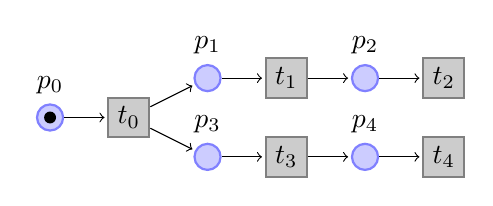
\begin{tikzpicture}
    \node[place,tokens=1] (p0) [label=above:$p_0$] {};
		\node[place] (p1) [right of=p0, xshift=1cm, yshift=0.5cm, label=above:$p_1$] {};
		\node[place] (p2) [right of=p1, xshift=1cm, label=above:$p_2$] {};

		\node[place] (p3) [right of=p0, xshift=1cm, yshift=-0.5cm, label=above:$p_3$] {};
		\node[place] (p4) [right of=p3, xshift=1cm, label=above:$p_4$] {};

    \node [transition] (t0) [right of=p0] {$t_0$}
				  edge [pre] (p0)
          edge [post] (p1)
					edge [post] (p3);
    \node [transition] (t1) [right of=p1] {$t_1$}
				  edge [pre] (p1) edge [post] (p2);
    \node [transition] (t2) [right of=p2] {$t_2$}
				  edge [pre] (p2);
    \node [transition] (t3) [right of=p3] {$t_3$}
				  edge [pre] (p3) edge [post] (p4);
    \node [transition] (t4) [right of=p4] {$t_4$}
				  edge [pre] (p4);
  \end{tikzpicture}
	\caption{Processus concurrents}
	\label{fig:origami}
\end{figure}

% ----- Exercice 2 -------------------- %

\section{Épicuriens ($\bigstar\bigstar\bigstar$)}

Le réseau de la figure \ref{fig:philo} représente le problème des philosophes pour un nombre $n$ de philosophes égal à $3$.

\begin{enumerate}
    \item Pliez le réseau pour éliminer les redondances entre les philosophes.
    \item Comment pourriez-vous étendre le modèle de réseau coloré obtenu au point 1 pour qu'il représente le problème des philosophes avec $n=100'000$ ?
\end{enumerate}

\begin{figure}[ht]
	\centering
  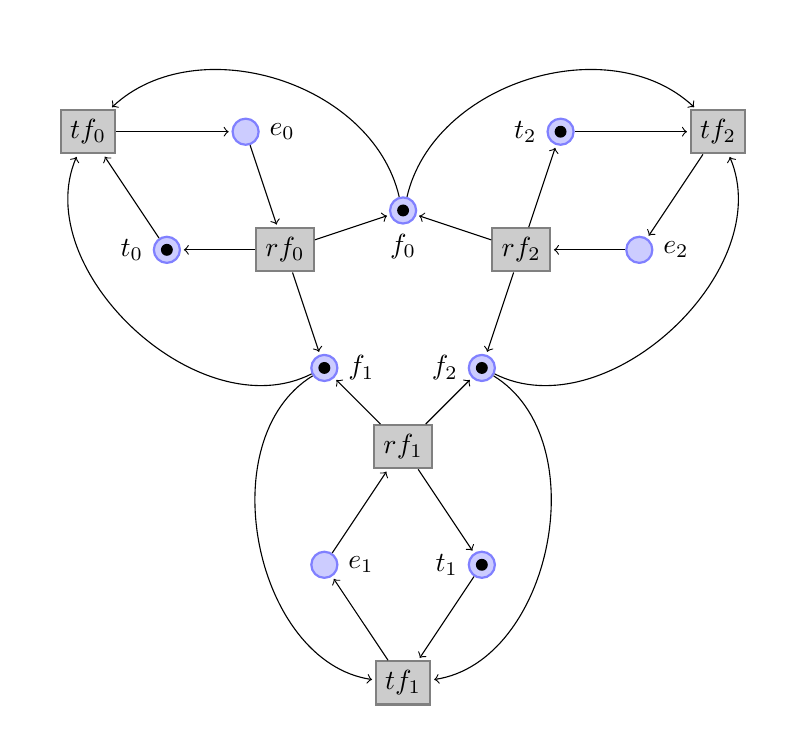
\begin{tikzpicture}
    % Forks:
    \node[place, tokens=1] (f0) [label=below:$f_0$] {};
    \node[place, tokens=1] (f1) [below of=f0, xshift=-1cm, yshift=-1cm, label=right:$f_1$] {};
    \node[place, tokens=1] (f2) [below of=f0, xshift=1cm, yshift=-1cm, label=left:$f_2$] {};
    
    % Philo 0:
    \node[place, tokens=1] (t0) [left of=f1, xshift=-1cm, yshift=1.5cm, label=left:$t_0$] {};
    \node[place] (e0) [left of=f0, xshift=-1cm, yshift=1cm, label=right:$e_0$] {};
    
    \node[transition] (rf0) [left of=f0, xshift=-0.5cm, yshift=-0.5cm] {$rf_0$} edge [pre] (e0) edge [post] (t0) edge [post] (f0) edge [post] (f1);
    \node[transition] (tf0) [left of=e0, xshift=-1cm] {$tf_0$} edge [pre, bend left=60] (f0) edge [pre, bend right=70] (f1) edge [pre] (t0) edge [post] (e0);
    
    % Philo 2:
    \node[place, tokens=1] (t2) [right of=f0, xshift=1cm, yshift=1cm, label=left:$t_2$] {};
    \node[place] (e2) [right of=f2, xshift=1cm, yshift=1.5cm, label=right:$e_2$] {};
    
    \node[transition] (rf2) [right of=f0, xshift=0.5cm, yshift=-0.5cm] {$rf_2$} edge [pre] (e2) edge [post] (f0) edge [post] (f2) edge [post] (t2);
    \node[transition] (tf2) [right of=t2, xshift=1cm] {$tf_2$} edge [pre, bend right=60] (f0) edge [pre, bend left=70] (f2) edge [pre] (t2) edge [post] (e2);
    
    % Philo 1:
    \node[place, tokens=1] (t1) [below of=f2, yshift=-1.5cm, label=left:$t_1$] {};
    \node[place] (e1) [below of=f1, yshift=-1.5cm, label=right:$e_1$] {};
    
    \node[transition] (rf1) [below of=f1, xshift=1cm] {$rf_1$} edge [pre] (e1) edge [post] (f1) edge [post] (f2) edge [post] (t1); 
    \node[transition] (tf1) [below of=e1, xshift=1cm, yshift=-0.5cm] {$tf_1$} edge [pre, bend left=70] (f1) edge [pre, bend right=70] (f2) edge [pre] (t1) edge [post] (e1);
  \end{tikzpicture}
	\caption{Modèle à 3 philosophes}
	\label{fig:philo}
\end{figure}

\end{document}
